\documentclass{article}

\usepackage[utf8]{inputenc}
\usepackage[german]{babel}
\usepackage[
    a4paper, top=2.5cm, bottom=2.5cm, left=2.5cm, right=2.5cm, marginparwidth=1.75cm
]{geometry}
\usepackage{amsmath}
\usepackage{amsfonts}
\usepackage{enumitem}
\usepackage[
    colorlinks=true, 
    citecolor=black,
    filecolor=black,
    linkcolor=black,
    urlcolor=blue
]{hyperref}
\usepackage{graphicx}
\usepackage{amssymb}
\usepackage{float}
\usepackage{siunitx} \sisetup{locale = DE}
\usepackage{pdfpages}
\usepackage{multirow}
\usepackage[
    tocskip=0.1\baselineskip, skip=0.7\baselineskip, parfill
]{parskip}
\usepackage{listings}
\usepackage{fancyhdr}
\usepackage{xcolor}

% Kopf- und Fußzeile
\pagestyle{fancy}
\fancyhf{}
%Kopfzeile mittig mit Kaptilname
\fancyhead[C]{\nouppercase{\leftmark}}
%Fußzeile links bzw. innen
\fancyfoot[L]{\versuchsname}
%Fußzeile mittig (Seitennummer)
\fancyfoot[R]{\thepage}
\renewcommand{\footrulewidth}{0.35pt}

% Hilfs-Commands für Gleichungen
\newcommand{\widespace}{\enspace}
\newcommand{\wideeq}{\widespace = \widespace}
\newcommand{\wideneq}{\widespace \neq \widespace}
\newcommand{\wideapprox}{\widespace \approx \widespace}
\newcommand{\wideleq}{\widespace \leq \widespace}
\newcommand{\widegeq}{\widespace \geq \widespace}
\newcommand{\widele}{\widespace \le \widespace}
\newcommand{\widege}{\widespace \ge \widespace}
\newcommand{\wideiff}{\widespace \iff \widespace}
\newcommand{\wideimplies}{\widespace \implies \widespace}
\newcommand{\pd}[2]{
    \frac{\partial #1}{\partial #2}
}
\newcommand{\result}[2]{
    #1 \, \text{#2}
}

% Markieren von verwendetem Code
\definecolor{codebg}{RGB}{230, 240, 255}
\newcommand{\coderef}[1]{%
    \text{\footnotesize \colorbox{codebg}{\texttt{#1()}}}%
}

% Formatieren von Code im Anhang
\definecolor{codegreen}{rgb}{0,0.6,0}
\definecolor{codegray}{rgb}{0.5,0.5,0.5}
\definecolor{codepurple}{rgb}{0.58,0,0.82}
\definecolor{backcolour}{rgb}{0.95,0.95,0.92}
\lstdefinestyle{mystyle}{
    backgroundcolor=\color{backcolour},   
    commentstyle=\color{codegreen},
    keywordstyle=\color{magenta},
    numberstyle=\tiny\color{codegray},
    stringstyle=\color{codepurple},
    basicstyle=\ttfamily\footnotesize,
    breakatwhitespace=false,         
    breaklines=true,                 
    captionpos=b,                    
    keepspaces=true,                 
    numbers=left,                    
    numbersep=5pt,                  
    showspaces=false,                
    showstringspaces=false,
    showtabs=false,                  
    tabsize=4
}
\lstset{style=mystyle}

% Formatierung von Absätzen
\renewcommand{\baselinestretch}{1.2}

\allowdisplaybreaks

% Allgemeine Infos
\newcommand{\versuchsname}{
    PLP - Plasmaphysik
}
\newcommand{\githuburl}{
    \url{https://github.com/WeinSim/P3B}
}

% Titel und Autor
\title{\versuchsname}
\author{Simon Weinzierl, Yannic Werner}

\begin{document}

\maketitle

\begin{center}
    Physikalisches Fortgeschrittenenpraktikum P3B
    nach der Studienordnung für Studienbeginn bis WS 2022/23
\end{center}

\vspace*{6cm}

\begin{center}
    \footnotesize
    Alle Teile dieses Dokuments (Vorbereitung, Protokoll, Auswertung) wurden
    von beiden Teilnehmern in gleichen Teilen und ohne fremde Hilfe bearbeitet.
    Sofern fremde Quellen verwendet wurden, sind diese angegeben.

    Der \LaTeX-Code ist auf GitHub unter \githuburl verfügbar.
    
    © Alle Rechte vorbehalten.
\end{center}

 % LMU-Siegel
\AddToShipoutPicture*{
    \put(315,0){
        \parbox[b][5cm]{5cm}{
            
\includegraphics[width=10cm]{Abbildungen/Siegel_LMU.pdf}
        }
    }
}

\newpage

% Inhaltsverzeichnis
\tableofcontents

\newpage

% Literatur
\bibliographystyle{alpha}
\bibliography{literatur}

\newpage

\section{Vobereitung}

\subsection{Physikalischer Hintergrund}

\subsubsection{Plasma}

\cite[1356]{Physik}

\cite{MPG}

Als Plasma bezeichnet man den vierten Aggregatzustand der Materie. Wenn man die Aggregatzustände der Materie aufzählen möchte, so folgt nach fest, flüssig und gasförmig der vierte Zustand, Plasma. Diesen Zustand erreicht mein, wenn man Materie immer weiter erhitzt bis schließlich ein Gas aus weitgehend frei beweglichen positiven Ionen und Elektronen entsteht. Dabei sind cairca 99 Prozent der ganzen Materie im Universum Plasma. Dies liegt daran, dass alle Sterne aus sehr heißem, ionisierten Gas bestehen, was als Plasma bezeichnet wird. Dieses Gas bildet schlussendlich auch die Grundlage für alle Sterne, damit sie durch Kernfusion Energie gewinnen können. 

Die Eigenschaften von Plasma unterscheiden sich jedoch von den klassichen Eigenschaften eines herköm- mlichen Gases. Zum einen ist Plasma leitend und kann zum anderen durch magnetische und elektrische Felder beeinflusst werden. Dies macht sich die Wissenschaft zu Nutzen und versucht auf Basis dessen mit Hilfe der Plasmaphysik einen Weg zu finden, wie man aus der Verschmelzung von Atomkernen Energie gewinnen kann. 

\subsubsection{Klassifizierung von Plasmen}

\cite[15--20]{Pp} 

\cite[14--16]{EidPp} 

\cite{PMT}

Plasmen lassen sich grob in fünf Kategorien einteilen. Im Folgenden sollen die jeweiligen Kategorien genauer beleuchtet werden.
\begin{enumerate}
    \item Ideales / nicht ideales Plasma: hierbei vergleicht man die potentielle Energie zwischen zwei Ladungsträgern mit der thermischen Energie. Ergibt dieser Vergleich, dass die thermische Energie deutlich höher ist als die potentielle Energie, so spricht man von einem idealen Plasma. Dabei ist der Begriff des idealen Plasmas an die Bezeichnung des idealen Gases angelehnt. Folglich kann man bei einem idealen Plasma die Wechselwirkungen zwischen den Teilchen (Coulombvwechselwikungen) vernachlässigen. Es gelten folgich für das ideale Plasma die allgemeinen Gasbedingungen für den Druck und die innere Dichte der Energie. Mathematisch lässt sich als Bedingung für das ideale Plasma folgende Gleichung aufstellen:
    
   \[
       \frac{3}{2} kT \widege \frac{e^2}{4\pi\varepsilon_{0}} n^{1 / 3}
       \quad \to \quad T[\unit{\eV}] \widege
       \left( \num{.79e-9} n [\unit{\per\cubic\meter}] \right)^{1 / 3}
   \]

   Bei einem nicht idealen Plasma ist die potentielle Energie zwischen den beiden Ladungsträgern größer ist als die thermische Energie.

   \item Ionisationsgrenze: die Ionisationsgrenze beschreibt den unteren Bereich, in welchen Plasmen existieren können. Der Ionisations- / Ionisierungsgrad lässt sich über folgende Formel bestimmen

   \[   
       X \wideeq \frac{n_{e}}{n_{e}+n_{0}},
   \]

    wobei $n_{0}$ die Dichte der neutralen Teilchen beschreibt. 

    \item Relativistische Grenze: diese Art der Betrachtung muss verwendet werden, sofern die thermische Energie der Elektronen die Ruhemasse von \qty{511}{\keV} überschreitet. In solchen Plasmen darf die Relativitätstheorie folgich zur Beschreibung nicht außer Acht gelassen werden. Der Effekt der Teilchenerzeugung / -vernichtung kann zudem aufgrund von außreichender Energie eintreten. Auch thermische Plasmen können breits solche Effekte aufweisen, jedoch werden die relativistischen Effekte hier nicht berücksichtigt.

    \item Entartung: erreicht man sehr hohe Dichen, so sind quantenmechanische Aspekte nicht zu vernachlässigen. Abgeleitet aus dem  muss die Zahl der möglichen quantenmechanischen Zustände folglich abgezählt werden. Es ergbit sich für die möglichen Zustände folgende Formel: 
    \[
        dN \wideeq 2\frac{L}{\pi\hbar}^3 d^3p
        \wideeq 2 \frac{4\pi}{(\pi\hbar)^3} p^2 \, dp
    \]

    Die Besetzungsdichte $n$ ist gegeben durch
    \[
        n \wideeq \int_{0}^{N/V} \, dN
        \wideeq \int_{0}^{E_\text{max}} g(e) \,dE
        \wideeq \frac{2}{3\pi^2} \frac{\sqrt{2m^3}}{\hbar^3} (E_\text{max})^{3/2}
    \]

    $E_\text{max}$ wird dabei auch als Fermi-Energie bezeichnet, welche sich mathematisch folgend ausdrücken lässt:
    \[
        E_\text{F} \wideeq \frac{\hbar^2}{2m} (3\pi^2)^{3/2} n^{3/2}
    \]

    \item Relativistische Entartung: diese Grenze ist definiert für den Fall, dass die Fermi-Energie die relativistische Energie überschreitet. Hierfür ergibt sich eine neue Formel der Energie, da man beachten muss, dass sich die Energie-Impuls-Beziehung ändert:
    \[
        E_\text{F, rel} \wideeq p_\text{F} c \wideeq \hbar c (3\pi^2)^{1/3} n^{1/3}
    \]
    
\end{enumerate}

Zusammenfassend hat man bei der Klassifizierung von Plasmen also folgende Aspekte zu beachten:
\begin{itemize}
    \item Ideales/nicht ideales Plasma
    \item Ionisationsgrenze
    \item Relativistische Grenze
    \item Entartung
    \item Relativistische Entartung
\end{itemize}

Möchte man nun verschiedene Plasmen klassifizieren und in Kategorien einordnen, so ergeben sich folgende Möglichkeiten:
\begin{enumerate}
    \item Klassifizeirung nach Druck: dabei differenziert man zwischen Niederdruck-Plasmen, Athmosphär- ischen Druckplasmen und thermischen Hochdruck-Plasmen.
    \item Klassifizierung nach Temperatur: hierbei unterscheidet man zwischen Kalt- und Heißplasma
    \item Alle oben erwähnten Aspekte und Unterscheidungsarten
\end{enumerate}


\subsubsection{Vakuum}

Ein Vakuum in einem Volumen liegt dann vor, wenn der Druck in dem Volumen
deutlich unter dem Umgebungsdruck, d.h. dem Atmosphärendruck liegt.
Dies kommt dadurch zustande, dass fast alle Gasmoleküle das Volumen verlassen
haben. Der maximal erreichbare Vakuumdruck hängt von der verwendeten Vakuumpumpe
sowie von den Oberflächen der Innenwände ab.

\cite[268]{demtröder}


\subsubsection{Klassifizierung von Vakua}

Ein Vakuum wird je nach dem vorherrschenden Druck einer von vier Kategorien
zugeordnet:
\begin{itemize}
    \item $\qty{1}{hPa} \leq p \leq \qty{1000}{hPa}$: Grobvakuum.
    \item $\qty{1e-3}{hPa} \leq p \leq \qty{1}{hPa}$: Feinvakuum.
    \item $\qty{1e-7}{hPa} \leq p \leq \qty{1e-3}{hPa}$: Hochvakuum.
    \item $p \leq \qty{1e-7}{hPa}$: Ultrahochvakuum.
\end{itemize}
Ein wesentlicher qualitativer Unterschied zwischen Fein- und Hochvakuum ist das
Verhältnis aus der mittleren freien Weglänge eines Teilchens zur
zur typischen Größe eines Vakuumgefäßes. In einem Feinvakuumbereich ist die mittlere
freie Wegläne, d.h. die mittlere Distanz, die ein Teilchen aufgrund seiner
thermischen kinetischen Energie zurücklegt, bevor es mit einem anderen Teilchen
zusammenstößt, sehr viel kleiner als die Gefäßgröße.
Im Hochvakuumbereich ist die Teilchendichte geringer als im Feinvakuumbereich.
Dadurch wird die mittlere freie Weglänge größer als die Gefäßgröße und die Teilchen
schweben nahezu kollisionsfrei im Raum umher.

\cite[268--269]{demtröder}


\subsubsection{Auger-Meitner-Effekt}

Grundlage für das Auftreten des Auger-Meitner-Effekts ist ein unbesetzter
Elektronenzustand in einem inneren Orbital eines Atoms.
Wird dieser von einem äußeren Elektron besetzt, dann gibt dieses die Energiedifferenz
in Form eines Photons ab. Dieses Photon kann direkt wieder von einem anderen
Elektron in diesem Atom absorbiert werden. Ist die Energie des Photons hoch
genug, dann kann das andere Elektron (genannt das Auger-Elektron) dem Atom
entweichen, wodurch dieses ionisiert wird.

\cite{Ossila}


\subsubsection{Teslatransformator}

Ein Teslatransformator ist ein Transformator, mit dem sehr hochfrequente
Wechselspannungen erzeugt werden können.
Er besteht im Wesentlichen aus zwei magnetisch gekoppelten elektromagnetischen
Schwinkreisen mit einem sehr großen Windungszahlverhältnis, d.h. $N_2 \gg N_1$,
wobei $N_1$ und $N_2$ die Windungszahlen der Primär- bzw. Sekundärspule sind.
Weil das Verhältnis von Primär- zu Sekundärspannung in einem Transformator
gleich dem Verhältnis der Windungszahlen der Primär- und Sekundärspulen ist,
wird in der Sekundärspule eine sehr hohe Spannung induziert.
Wichtig dabei ist, dass die beiden Schwingkreise dieselbe Eigenfrequenz besitzen.

\cite{leifi_tesla}


\subsubsection{Funktionsweise einer Drehschieberpumpe}

Mit folgender Abbilung soll das Prinzip und die Funktionsweise der Drehschieberpumpe erklärt werden:

\begin{figure}[H]
    \centering
    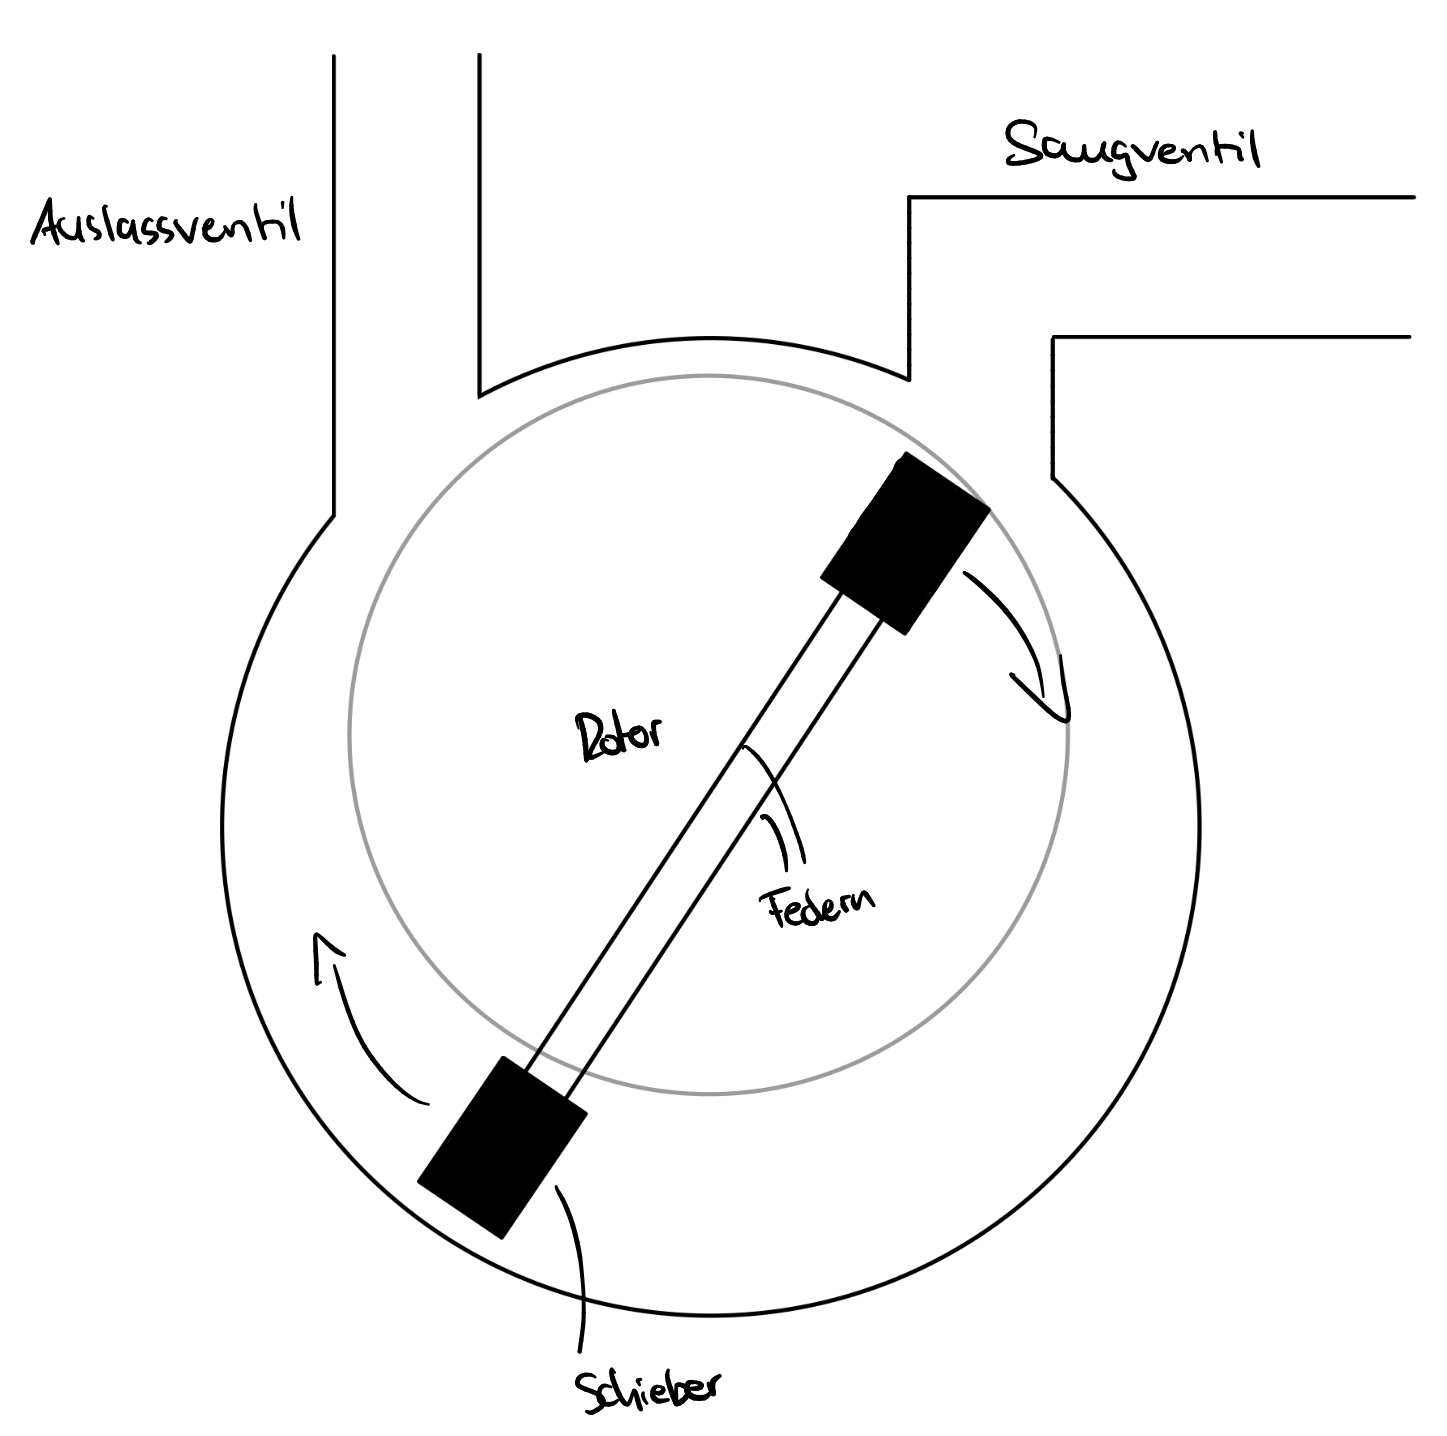
\includegraphics[width=0.5\linewidth]{Abbildungen/Drehschieberpumpe.jpeg}
    \caption{Darstellung einer Drehschieberpumpe}
\end{figure}

Zu Beginn strömt Luft über das Saugventil in den Zylinder der Drehschieberpumpe. Sobald sich der Rotor bewegt, gleiten die beiden Schieber entlang der Zylinderwand und schieben dadurch das Gas vor sich her. Dadurch wird das Gas komprimiert und schließlich in den Auslass gedrückt. Die beiden Schieber werden durch zwei Federn auseinandergedrückt, damit diese immer an der Wand entlang gleiten.

Das angeführte Beispiel ist eine einstufige Drehschieberpumpe. Hier herrscht am Auslasskanal immer Atmosphärendruck. Durch die Bewegung des Rotors entsteht am oberen Ende ein kleiner Spalt, durch welchen immer etwas Lust vom Auslasskanal zum Saugkanal fließt (Grund: Druckgefälle). Um diese Art von Verlusten zu vermeiden, füllt man die Pumpe zum Teil gerne mit Öl. Der so entstehende Film zwischen Rotor und Gehäuse dichtet die Pumpe dann ab. 

Durch die Kombination von mehreren Drehscheibepumpen kann man den Endtotaldruck erhöhen. Verwendet man beispielsweise zwei Pumpen hintereinander, spricht man von einer zweistufigen Drehschieberpumpe. Hierbei saugt die zweite Pumpe am Auslasskanal der ersten Pumpe.

\subsubsection{Eigene Skizze zur Funktionsweise einer Scrollpumpe}

\cite{vt}

Folgende Abbildung soll das Prinzip und die Funktionsweise von Scrollpumpen verdeutlichen. Dabei wurde eine Aufteilung in vier Schritte vorgenommen, welche im Folgenden genauer betrachtet werden. Die jeweils markierte Fläche stellt dabei den Verdichtungsgrad des Gases dar.

\begin{figure}[H]
    \centering
    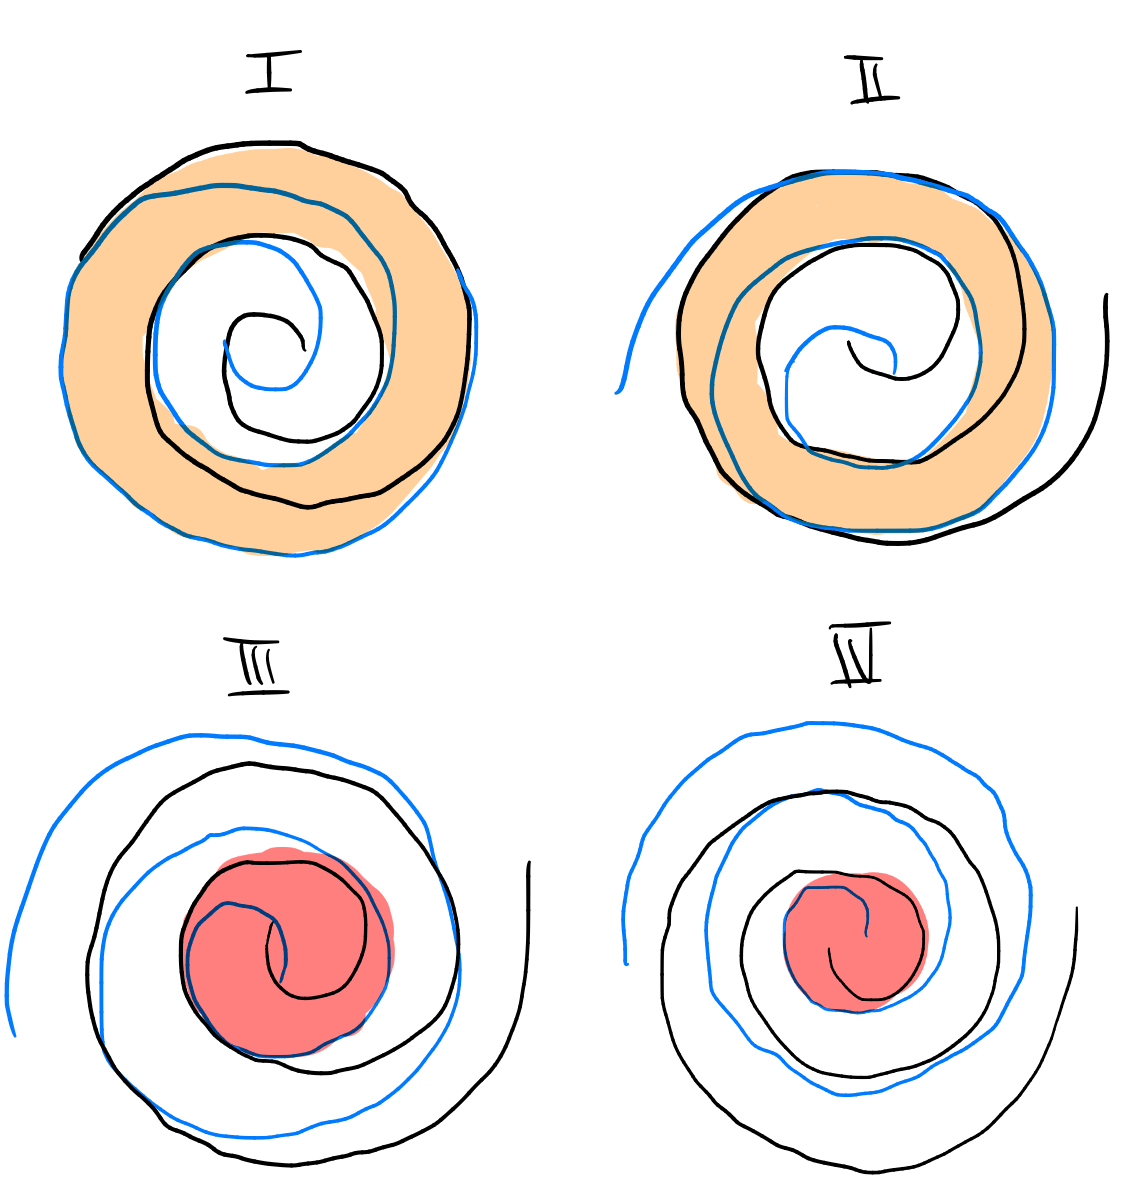
\includegraphics[width=0.5\linewidth]{Abbildungen/Scrollpumpe.jpeg}
    \caption{Funktionsweise einer Scrollpumpe}
\end{figure}

\begin{enumerate}[label = \Roman*.]
    \item Der Ansaaugvorgang ist beendet und das Gas ist in den Ansaugtaschen der Scrollpumpe eingeschlossen
    \item Die Komprimierung des Gases geht weiter voran und das Gas wird immer stärker verdichtet. Dabei drehen sich die Taschen der Scrollpumpe weiter und das eingeschlossene Gas wandert dabei immer weiter nach innen.
    \item Das Scrollen geht kontinuierlich weiter und das Gas bewegt sich immer weiter Richtung Mitte, währenddessen es immer weiter kompirmiert wird. Die Entaldung steht kurz bevor.
    \item Die Kompressionstaschen bewegen sich in die Mitte der Scrollpumpe. Das Gas ist maximal komprimiert und kann nun aus dem zentralen Ablassanschluss entweichen.
\end{enumerate}

Wie ersichtlich wandert das angesaugte Gas wie in einem Schneckenhaus nach innen, während es immer weiter komprimiert wird. Der Übergang von der orangen Farbe zur roten Farbe soll hierbei genau diesen Effekt darstellen, dass das Gas immer stärker verdichtet wird. Wird erneut Gas angesaugt, beginnt der Kreislauf von vorne.

\subsubsection{Vorteile von Scrollpumpen}

\cite{vt}

Im Folgenden sollen Vorteile der oben beschriebenen Scrollpumpe angeführt werden:

\begin{itemize}
    \item Wie bereits oben beschrieben, ermöglichen Scrollpumpen einen ununterbrochenen Fluss
    \item Man erreicht durch das ``stufenweise'' Verdichten von Gas eine sehr hohe Dichtheit des Gases
    \item Die Scrollpumpe ermöglicht einen verschmutzungsfreien Betrieb, da kein Schmiermittel verwendet wird
    \item Sie kann in jeder installierten Position arbeiten und benötigt keine spezielle Ausrichtung
    \item Zudem ist sie sehr leise und vibrationsarm, wodurch ein Versuchsaufbau unbeschädigt bleibt
    \item Sie haben eine hohe Effizienz, also eine hohe Pumpgeschwindigkeit
    \item Unabhängigkeit von Gasart
\end{itemize}

Diese Vorteile führen dazu, dass die Scrollpumpe ein beliebtes Beuteil ist, wenn man ein zuverlässiges und stabiles Vakuum erzeugen möchte. Gerade in der Physik bietet sich die Scrollpumpe daher an, da sie es ermöglich nahezu konstante Laborbedingungen zu erzeugen, in welchen anschließend klare und eindeutige Beobachtungen gemacht werden können. Zusammenfassend ist die Scrollpumpe also ein sehr vielseitg einsetzbares Bauteil, welches es ermöglicht, physikalische Beobachtungen und Versuche besser durchzuführen.

\subsection{Aufgabe aus dem Text}

In der folgenden Abbildung ist die Funktion $f(x) = \frac{A (x - C)}{\ln (B (x - C))}$
im Wertebereich $x \in [0; 100]$ für zwei verschiedene Sets an Parameterwerten
geplottet.

\begin{figure}[H]
    \centering
    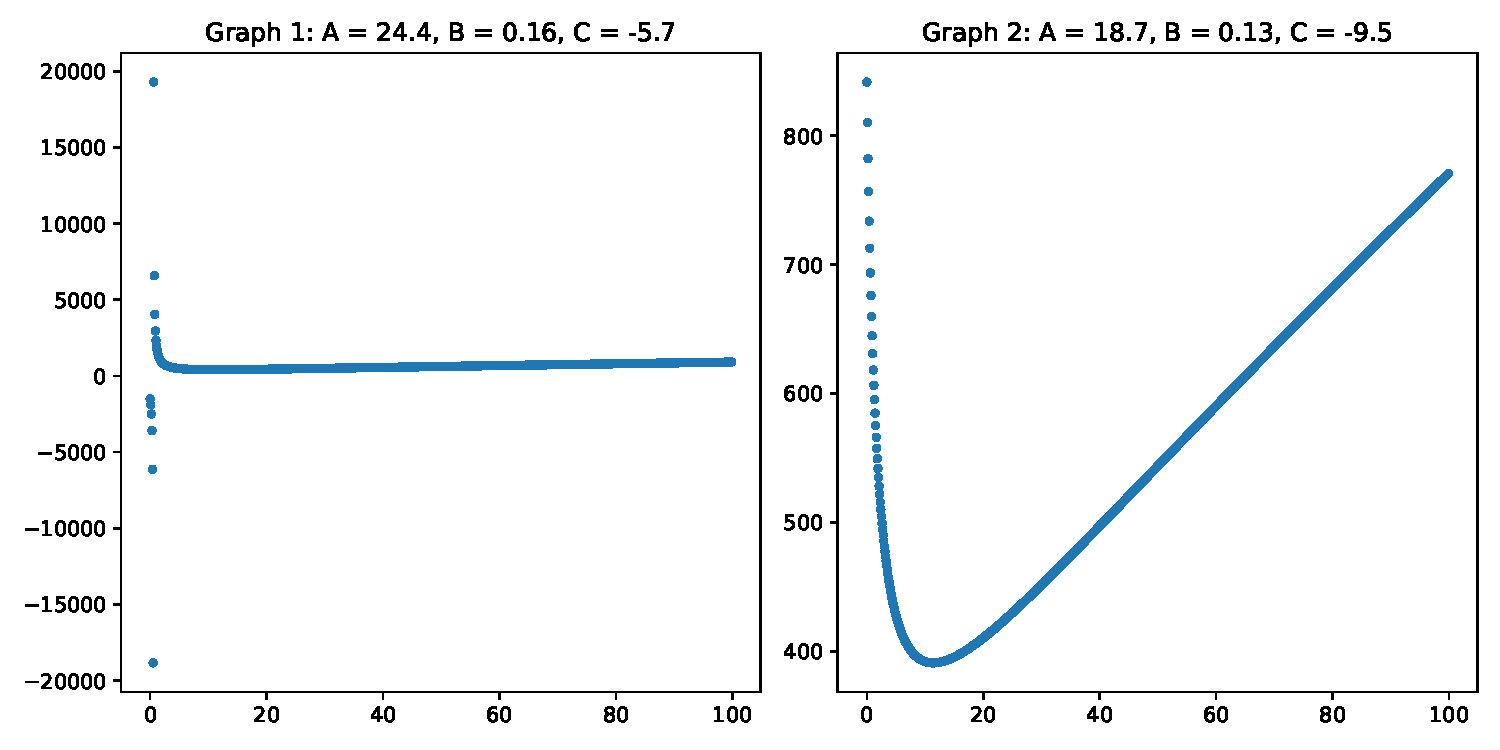
\includegraphics[width=0.95\linewidth]{Abbildungen/Graph_Vorbereitung.pdf}
    \caption{Funktionsplot der gegebenen Funktion für zwei verschiedene
    Parametersätze (\coderef{vorbereitung})}
\end{figure}

Der Parameter $A$ beschreibt die Streckung bzw. Stauchung des Graphs entlang der
$y$-Achse, weil der gesamte Ausdruck mit $A$ multipliziert wird.
Der Parameter $C$ beschreibt die Verschiebung entlang der $x$-Achse, weil $x$ immer
nur in Termen mit $x - C$ vorkommt.
Für $x = C + 1 / B$ wird das Argument des Logarithmus $1$ und damit der Nenner Null.
Also besitzt der Graph dort eine Singularität.
Der Parameter $B$ bestimmt das asymptotische Verhalten des Graphs in der Nähe der
Singularität.

Im ersten Parametersatz gilt $C + 1 / B = \num{.055}$, im zweiten gilt
$C + 1 / B \approx \num{-1.81}$ (\coderef{vorbereitung}).
Weil der Wert im ersten Satz positiv und im zweiten negativ ist, ist die Polstelle
im linken Graphen sichtbar und im rechten nicht.
Wegen der sichtbaren Polstelle im geplotteten Wertebereich wurden einzelen Punkte
anstatt einer kontinuierlichen Linie zum Plotten verwendet. Bei letzterer würden
die Datenpunkte direkt links bzw. rechts von der Polstelle miteinander verbunden
werden, was mathematisch nicht korrekt ist.


\newpage

\section{Veruschsablaufplan}

\subsection{Benötigte Materialien}
    \subsubsection{Teilversuch 1: Paschen-Kurve}
        \begin{enumerate}[label=\arabic*.]
            \item Plasmaphysik Betriebsgerät
            \item Plasmaphysik Experimentierset
            \item Digitalmultimeter mit Haltefunktion, Messbereich 1000V
            \item Mini DIN Verbindungskabel
            \item Erdungskabel
            \item 2x Messkabel, 32A
            \item Drehscheibenvakuumpumpe beziehungsweise Scrollpumpe
            \item Pirani-Vakuummeter
            \item Ölnebelfilter
            \item Nadelventil
            \item Vakuumschläuche, $d_{i}=8mm$
            \item Schlauchverbindungsstück, $d_{i}=8mm-9mm$
            \item 2x Kammerflansch
            \item 3x Spannring
        \end{enumerate}
    \subsubsection{Teilversuch 2: Oberflächenbehandlung}
        \begin{enumerate}[label=\arabic*.]
            \item Plasmaphysik Betriebsgerät
            \item Plasmaphysik Experimentierset
            \item Digitalmultimeter mit Haltefunktion, Messbereich 1000V
            \item Mini DIN Verbindungskabel
            \item Erdungskabel
            \item verschiedene Probekörper (Kunststoffe, Metalle) mit maximaler Dicke 1,5mm
            \item Eppendorf Mikropipette, $2\mu l-20\mu l$
            \item Pipettenspitzen
            \item Ethanol
            \item Ionisiertes Wasser
            \item Millimeterpapier
            \item LED Lampe
            \item CCD Kamera
            \item Kamerastatik
            \item Motic Software
            \item Measure Dynamics Software
            \item Rechner
        \end{enumerate}
    \subsubsection{Teilversuch 3: Plasmakugel}
        \begin{enumerate}[label=\arabic*.]
            \item Plasmakugel beziehungsweise Plasmaröhre
            \item Oszilloskopd mit Autosetfunktion
            \item Tastteiler
        \end{enumerate}

\newpage

\subsection{Teilversuch 1: Paschen-Kurve}
\begin{enumerate}[label = (\Roman*)]
    \item Ziel: Bestimmung der Paschen-Kurve
    
    \item Versuchsmethode: Die Zündspannung eines Niederdruckplasmas wird in Abhängigkeit von Druck und Elektrodenabstand bestimmt.
    
    \item Versuchsskizze:
    
        \begin{figure}[H]
        \centering
        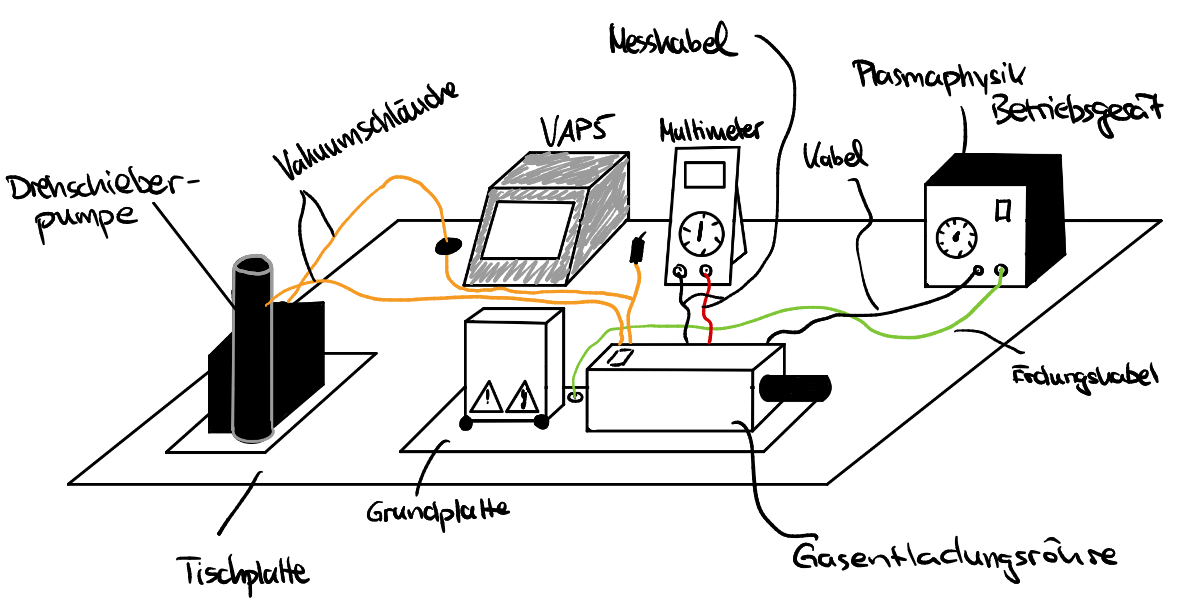
\includegraphics[width=0.7\linewidth]{Abbildungen/SkizzeTV1.jpeg}
        \caption{Versuchsskizze Teilversuch 1}
        \end{figure}

    \item Planung der Durchführung
        \begin{itemize}
            \item Das Nadelventil ganz aufdrehen und anschließend die Pumpe anschalten. Der Druck soll nun mittels Nadelventil auf einen Werte zwischen 2,5hPa und 6hPa eingestellt werden.
            \item Mittels der Mikrometerschraube soll der kleinstmögliche Abstand der Elektronen gewählt werden. 
            \item Das Steuergerät wird auf kontinuierlichen Betrieb eingestellt und der Spannungsregler wird bis zum Anschlag nach links gedreht.
            \item Das Multimeter wird konfiguriert.
            \item Das Plasmabetriebsgerät kann nun eingeschaltet werden
            \item Die Spannung wird langsam auf den maximal möglichen Wert erhöht. Anschließend soll der Elektronenabstand so lange erhöht werden, bis eine Glimmladung im Fenster sichtbar wird.
            \item Der Elektronenabstand wird auf $d = \qty{0}{\mm}$ rediziert. Er wird erneut bei maximaler Spannung vergrößert, bis eine Glimmspannungs erkennbar ist. Der Beginn des Durchbruchs stellt den Beginn der Messreihe dar (ab hier Entladung möglich!)
            \item Verfahren um Paschen-Kurve zu messen - Vorschlag: ermitteln der einzelnen Durchbruchsspannungen zu den einzelnen Elektronenabständen $\xrightarrow{}$ Spannung zwischen den beiden Elektroden wird kontinuierlich erhöht, bis eine Glimmladung einsetzt. Der gemesse Wert der Spannung kurz vor der Zündung wird notiert. Anschließend Auftragen der Wertepaare Spannung - Elektronenabstand.
            \item Beenden der Messung: Druck der Entladungsröhre langsam steigern (Öffnen von Nadelventil) $\xrightarrow{}$ automatisches Abschalten der Pumpe
        \end{itemize}

    \item Vorüberlegungen zur Durchführung \& Auswertung
        \begin{itemize}
             \item Drehschiebepumpe: Ölnebelfilter mit Pfeilrichtung von der Pumpe weg montieren!
             \item Es soll die Haltefunktion des Multimeters verwendet werden, da hier immer die kleinste und größte gemessene Spannung gespeichert werden. Relevant für die Messung ist immer der maximale Spannungswert, der einen Durchbruch ermöglicht.
             \item Mikrometerschraube mit Sorgfalt bedienen. Nicht überdrehen!
             \item Wichtig: Druck konstant halten!
             \item Mittelwerte der Elektrodenposition bilden!
             \item Auftragen gegen das Produkt aus Abstand und Druck!
             \item Messunsicherheiten nicht vergessen!
        \end{itemize}
    
\end{enumerate}

\newpage

\subsection{Teilversuch 2: Oberflächenbehandlung}
\begin{enumerate}[label = (\Roman*)]
    \item Ziel: Beschreiben der Veränderung der Oberflächenenergie
    
    \item Versuchsmethode: Die Benetzbarkeit eines Festkörpers mit einer Flüssigkeit wird mittels Oberflächenbehandlung durch ein Plasma verbessert. Daraus resultiert eine Veränderung des Kontaktwinkels eines Flüssigkeitstropfens.
    
    \item Versuchsskizze:
    
        \begin{figure}[H]
        \centering
        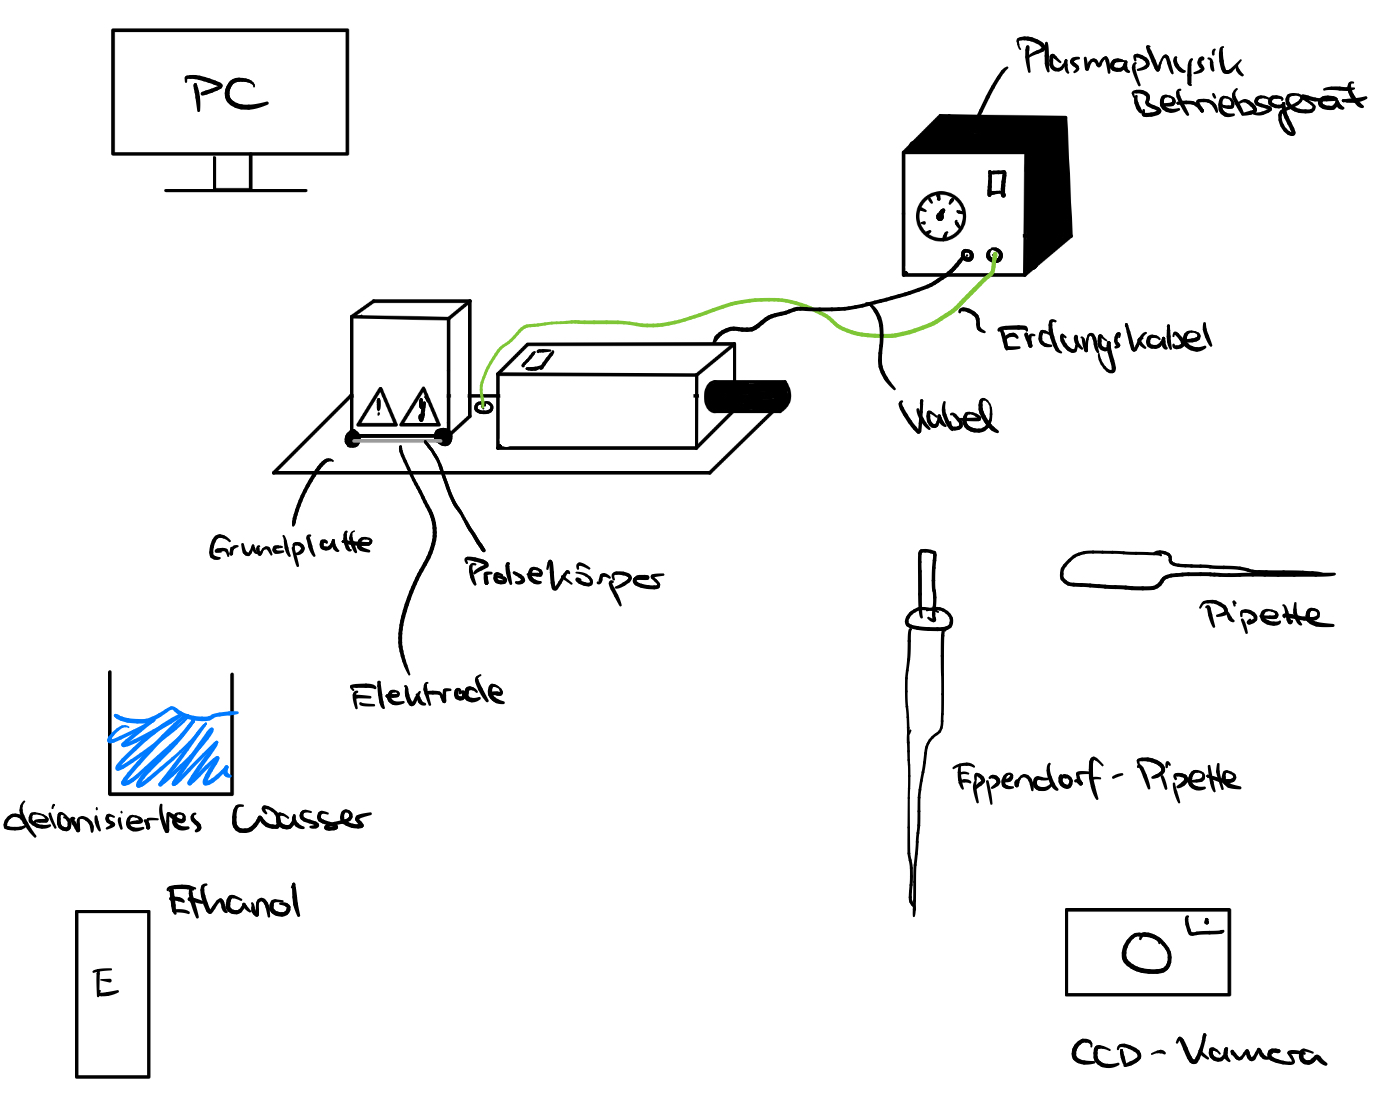
\includegraphics[width=0.7\linewidth]{Abbildungen/SkizzeTV2.jpeg}
        \caption{Versuchsskizze Teilversuch 2}
        \end{figure}

    \item Planung der Durchführung
        \begin{itemize}
           \item Betriebsgerät aktivieren und darauf achten, dass der Betriebsmodus auf ``Pulse'' und der Timer auf \qty{.2}{\s} gestellt ist
           \item Ausgewählten Probekörper mit Ethanol reinigen (maximale Dicke 1,5mm!)
           \item Den präparierten Probekörper unter die Elektrode legen und Einwirkzeit auswählen
           \item Anschließend dir Behandlung starten (Plasmaentladung wird akkustisch und optisch sichtbar)
           \item Nach Behandlung Probe beobachten (eventuelle Anhauchen, um Unterschiede erkennbar zu machen)
           \item Pipettenspitze auf Eppendorfä-Pipette stecken
           \item Auf beide Bereiche (behandelt und nicht behandelt) einen deionisierten Wassertropfen setzen ($V = \qty{2}{\ul}$)
        \end{itemize}

    \item Vorüberlegungen zur Durchführung \& Auswertung
        \begin{itemize}
            \item Vor dem Umbauen der Apparatur, immer das Netzteil trennen!
            \item Nur zugelassene Probekörper verwenden!
            \item Eppendorf-Pipette immer in Halterung verwahren, um Beschädigung zu vermeiden
            \item Vor jedem Gebrauch der Eppendorf-Pipette eine frische Spitze aufstecken
            \item Auswertung mittels Analyseprogramm am PC
            \item Probekörper auf Millimeterpapier legen und mit CCD Kamera Foto des Probekörpers aufnehmen
            \item Auswerten und Bestimmen des Konktaktwinkels mit der App $"$Measure Dynamics"
        \end{itemize}
        
\end{enumerate}

\newpage

\subsection{Teilversuch 3: Plasmakugel}
\begin{enumerate}[label = (\Roman*)]
    \item Ziel: Verstehen des Zustandekommend der Leuchterscheinungen innerhalb einer Plasmakugel
    
    \item Versuchsmethode: Beobachten der Leuchterscheinungen einer Plasmakugel sowie das hochfrequente Wechselfeld eines Teslatransformators.
    
    \item Versuchsskizze:
    
        \begin{figure}[H]
        \centering
        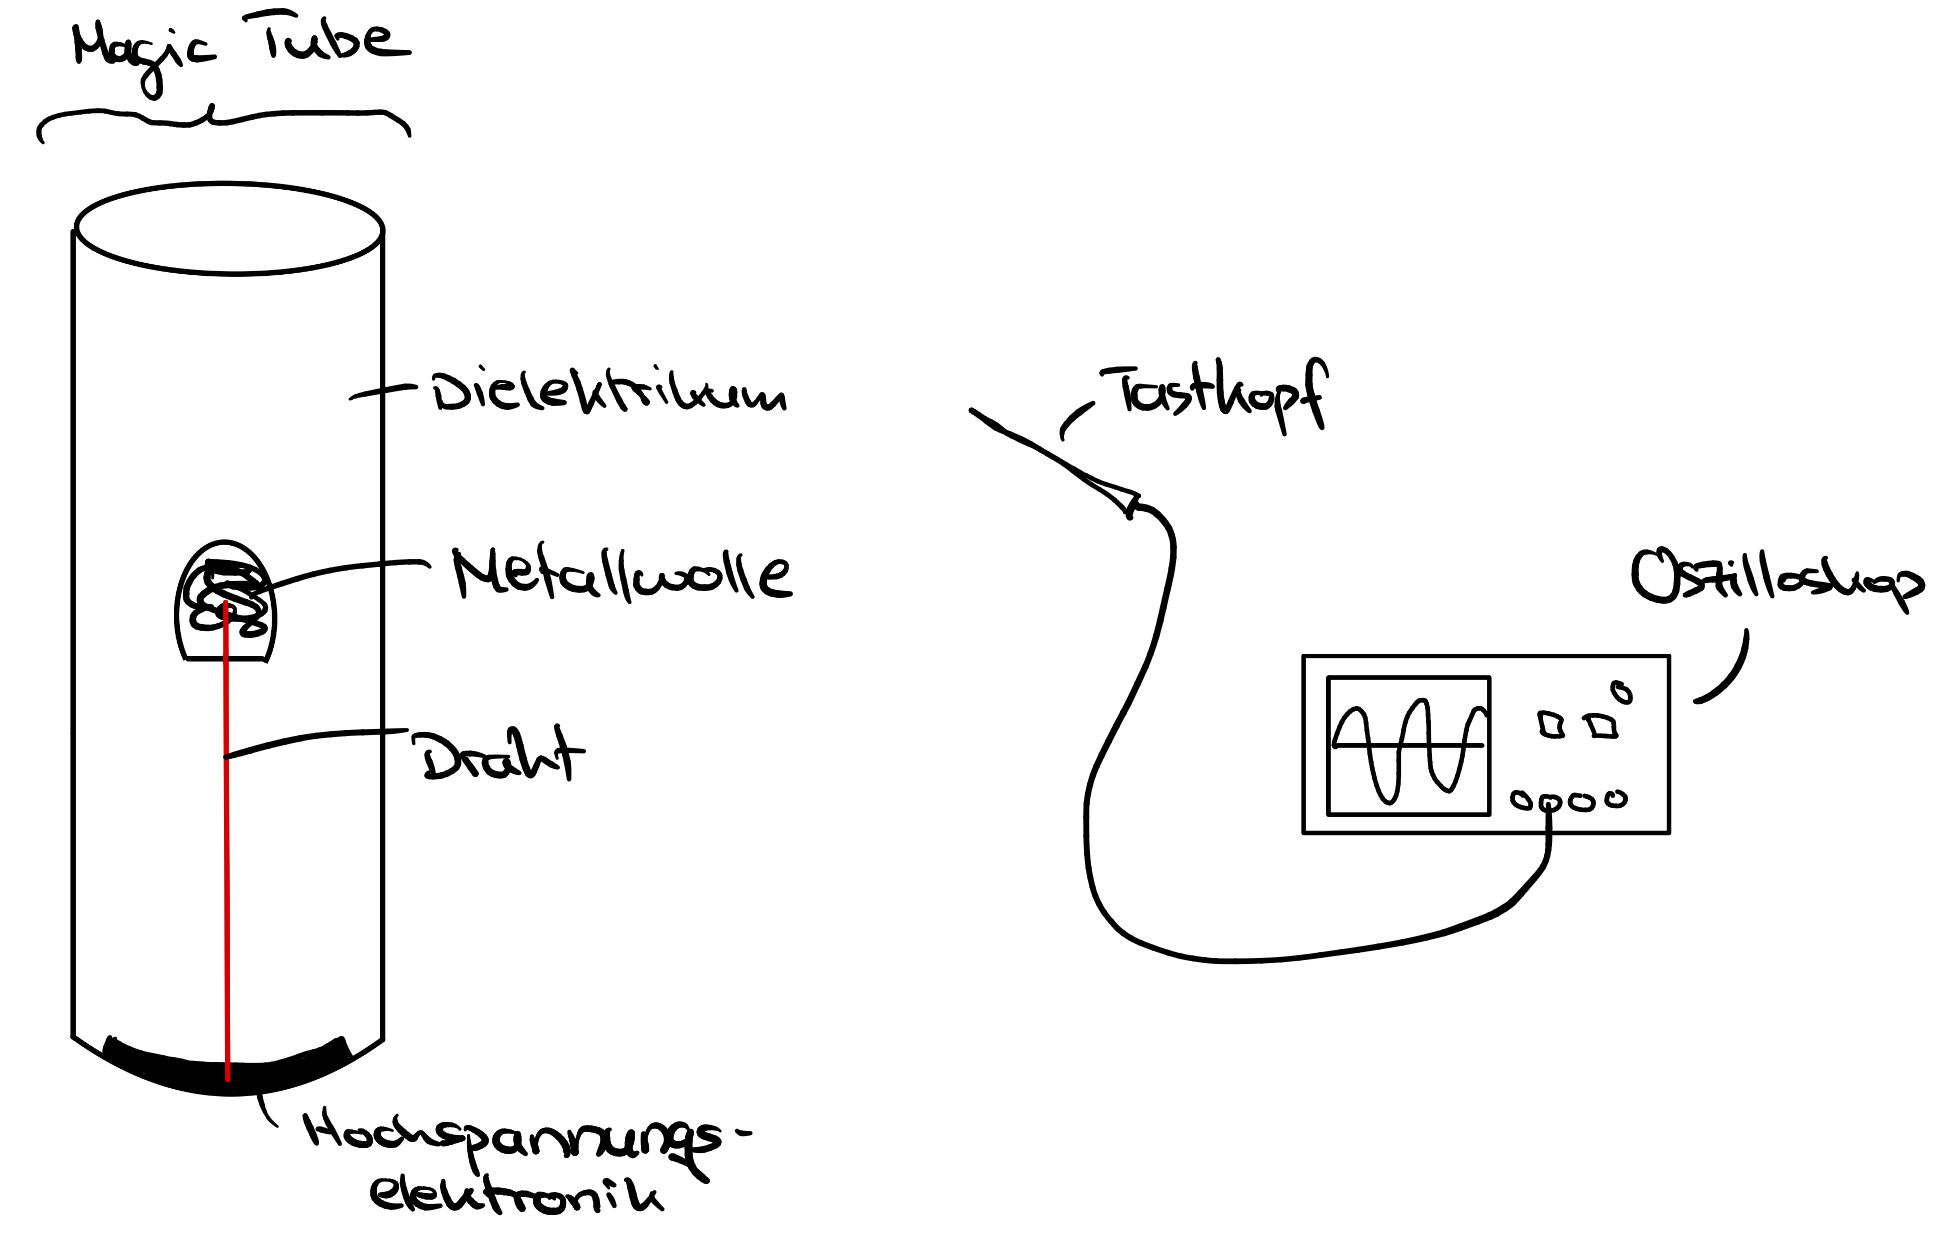
\includegraphics[width=0.7\linewidth]{Abbildungen/SkizzeTV3.jpeg}
        \caption{Versuchsskizze Teilversuch 3}
        \end{figure}

    \item Planung der Durchführung
        \begin{itemize}
           \item Plasmazylinder in Betrieg nehmen
           \item Beobachten der Plasmafäden mit und ohne Berührung der Oberfläche
           \item Bestimmen des Füllgases
           \item Bobachten des Felds der Lampe mit dem Tastkopf und dem Oszilloskopf an der Oberfläche und in einiger Entfernung
           \item Bestimmen der Frequenz des Teslatransformators
           \item Abstandsgesetz quantitativ untersuchen
        \end{itemize}

    \item Vorüberlegungen zur Durchführung \& Auswertung
        \begin{itemize}
            \item Keine Metalle und Flüssigkeiten auf die Oberfläche bringen. Es besteht Verbrennungsgefahr!
            \item Bestimmen eines Abstandsgesetzes zu den Messdaten
            \item Beschreiben und Darstellen durch Anpassung einer theoretischen Kurve
            \item Beschreiben von Plasma (Farbe)
            \item Frage: Warum bewegen sich die Plasmafäden?
        \end{itemize}
        
\end{enumerate}

\newpage

\iffalse

\section{Versuchsprotokoll}

Auf den folgenden Seiten befindet sich das eingescannte Versuchsprotokoll.
Alle Daten wurden selbst gemessen. Sofern fremde Hilfe benutzt wurde,
wurde sie klar gekennzeichnet.

Messunsicherheiten wurden angegeben und folgend in der Auswertung verwendet.
Alle weiteren Rechnungen und Analysen finden in der Versuchsasuwertung statt.

\includepdf[pages={...}, pagecommand={\thispagestyle{scrheadings}}, frame=true]{[Name.pdf]]}

\newpage

\section{Auswertung}

\subsection{Teilversuch 1: Bragg-Reflexion von Röntgenstrahlung des Molybdän an einem NaCl-Eiskristall}


\newpage

\fi

\section{Anmerkung: Graphische Auswertung und Fehlerfortpflanzung mit Python-Code}

Alle Berechnungen inkl. Fehlerbestimmung wurden Python durchgeführt, um uns die Arbeit
zu erleichtern und Fehler zu vermeiden.
Alle Ergebnisse, die auf diese Weise zustande gekommen sind,
sind entsprechend mit einem \colorbox{codebg}{blauen Hintergrund} gekennzeichnet;
s. folgendes Beispiel:
\[
    F \wideeq ma \wideeq \qty{20}{\kg} \cdot \qty{9.81}{\meter\per\square\second}
    \wideeq (\num{19.6} \pm \num{0,5}) \unit{\N} \widespace \coderef{tv1}
\]
Das bedeutet, dass die Berechnung des Wertes und der Unsicherheit von der
Python-Funktion namens \verb|tv1| durchgeführt wird.
Die Unsicherheit wird mithilfe der Gauß'schen Fehlerfortpflanzung berechnet.
Eine genauere Erklärung dazu befindet sich auf GitHub und in den Kommentaren im Code.
Außerdem wird das Package \texttt{matplotlib} zum Erstellen
von Graphen verwendet.

Der verwendete Code ist sowohl auf GitHub verfügbar (\githuburl) als auch auf den
folgenden Seiten zu finden und kann mit dem Befehl \texttt{python main.py}
ausgeführt werden. Für eine genauere Beschreibung des Codes siehe die README-Datei
auf GitHub sowie die Kommentare im Code.
(Manche Sonderzeichen im Code (ä, ö, ü, $\Delta$, etc.) werden von \LaTeX nicht
richtig erkannt, deswegen kann der Code auf den nachfolgenden Seiten an einigen
Stellen unvollständig erscheinen. Auf GitHub wird aber alles richtig angezeigt.)

\newpage


\verb|main.py|:
\lstinputlisting[language=Python]{Code/main.py}
\newpage

% \verb|Expressions.py|:
% \lstinputlisting[language=Python]{Code/Expressions.py}
% \newpage

Output:
\lstinputlisting{Code/output.txt}

\end{document}